\documentclass{article}
\usepackage{tikz}
\usepackage{graphicx}
\usepackage{hyperref}
\graphicspath{ {./img/} }

\author{Kent Odde, Stian Onarheim, Tarald Vestbøstad}
\title{Title}

\begin{document}

\pagestyle{empty}

 \begin{tikzpicture}[remember picture,overlay]
    \node[anchor=north west,yshift=-15pt,xshift=20pt]%
        at (current page.north west)
        {
\includegraphics[height=8em]{img/USN_logotype.png}};

\end{tikzpicture}


%\vspace{2.5cm}

{\LARGE test}\hspace{2cm}

\begin{tikzpicture}[overlay]
    \node[anchor=north, inner sep=0] at (4,-2)
        {
\includegraphics[width=\textwidth]{img/frontpage-block.png}};
\end{tikzpicture}

\begin{tikzpicture}[overlay]
    \node[anchor=north, inner sep=0] at (-3,-0) {\large Hello};
        
\end{tikzpicture}

\maketitle

\section{Maybe useful text}

Thursday 20. August 2020, the group gathered and had a meeting with Steven Bos. We discussed our project idea and the potential use of the Microsoft HoloLens 2. It was in the group's best interest to put our resources into the microcontroller rather than the goggles, dismissing any development with the HoloLens.

\vspace{5mm}
On September 10. the group met to plan the project. After deciding on the initial design, we drew a sketch and wrote a short description. This was sent to our professor, along with a list of required parts as well as the associated budget. The initial design can be seen in section XX.

\vspace{5mm}

On the 16th of September, we ordered three Arduino Nano BLE Sense from Arduino.cc. This came to 1080NOK. In addition to this the professor provided us with a car for the project. It is called \href{https://hobbyking.com/en_us/turnigy-trooper-sct-4x4-1-10-brushless-short-course-truck-arr.html?___store=en_us}{Turnigy Trooper}, and was originally a radio controlled car. However everything but the battery and servo motors for thrust and steering, have been stripped away. 

The servo motors are controlled by a pulse-width modulated signal. This means in essence that we send discrete signals, where the signal will rise at a fixed frequency. The length of time the signal is high before going low will determine the behaviour of the servo motors. Luckily for us there is a standard regarding the behaviour generated by a specific pulse width. 

We will need to write a library which will abstract this away in the code. Where the interface for steering will take an angle, and the motor interface will hopefully be able to take a velocity in m/s, where negative numbers will mean going backwards. 






\vspace{5mm}

Legge til utilization test og grafikk.

\section{Maybe useful pictures}

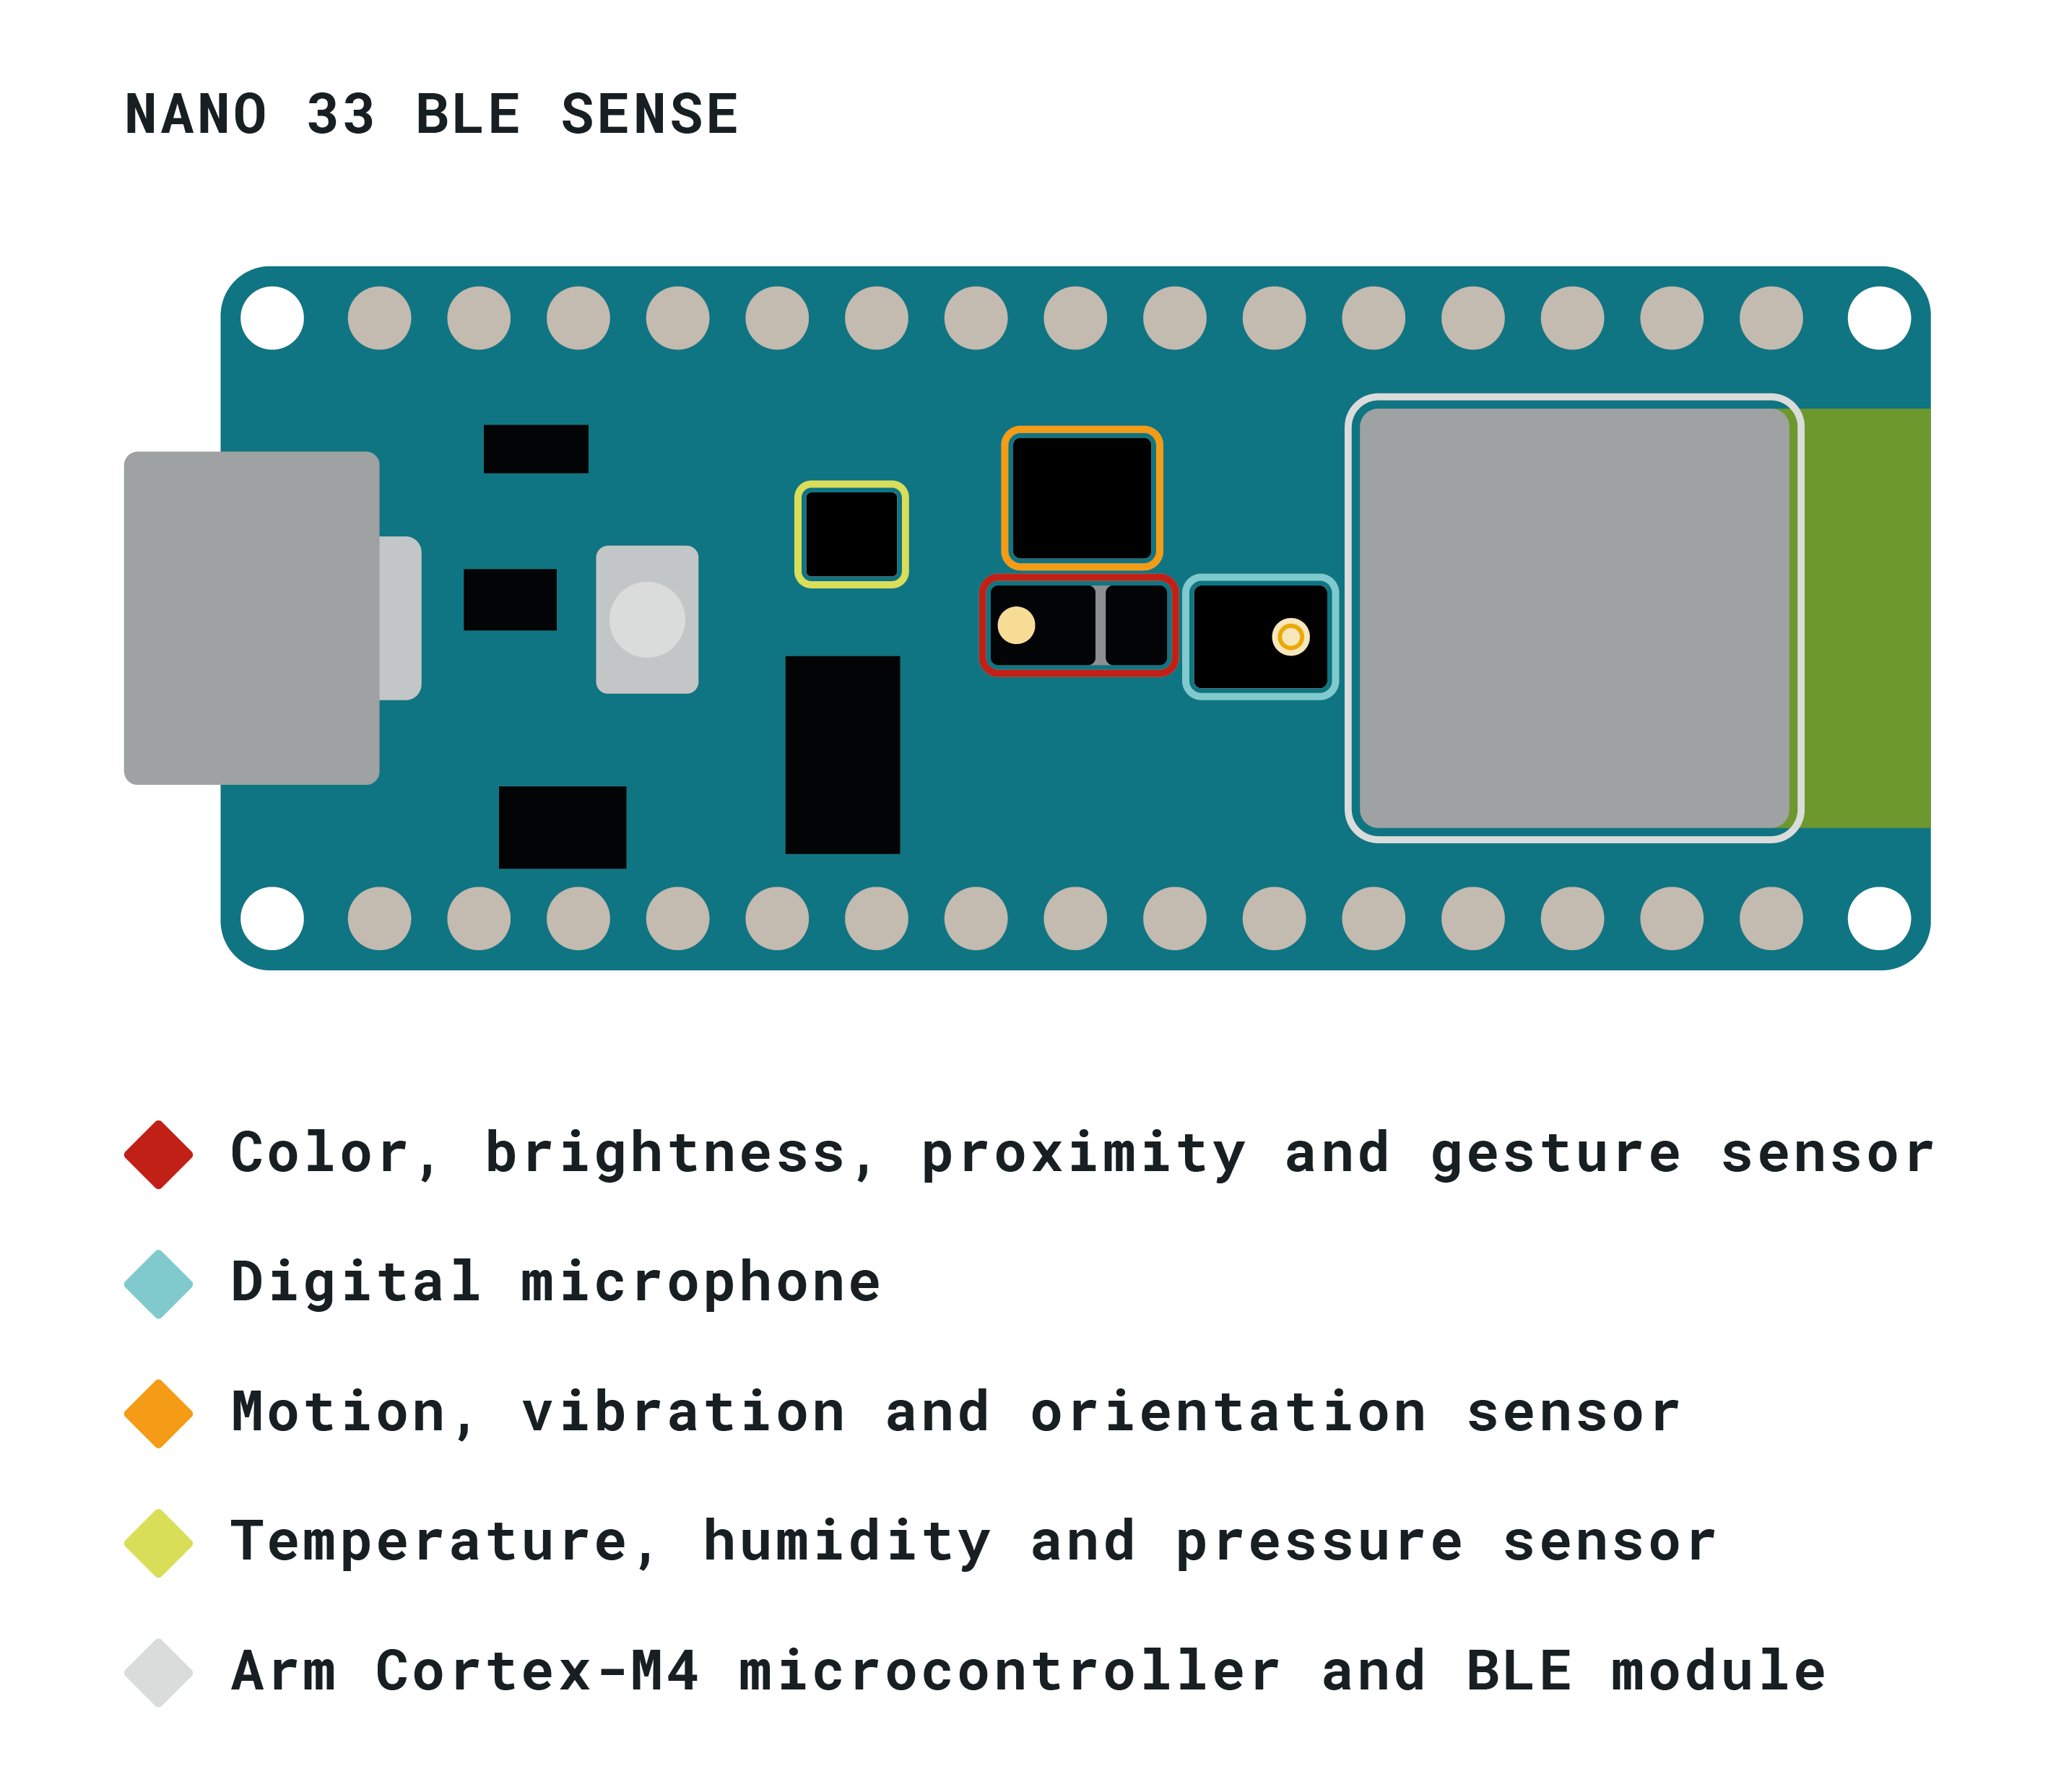
\includegraphics[width=\linewidth]{img/NANO-33-BLE-Sense_sensor-indentification.png}

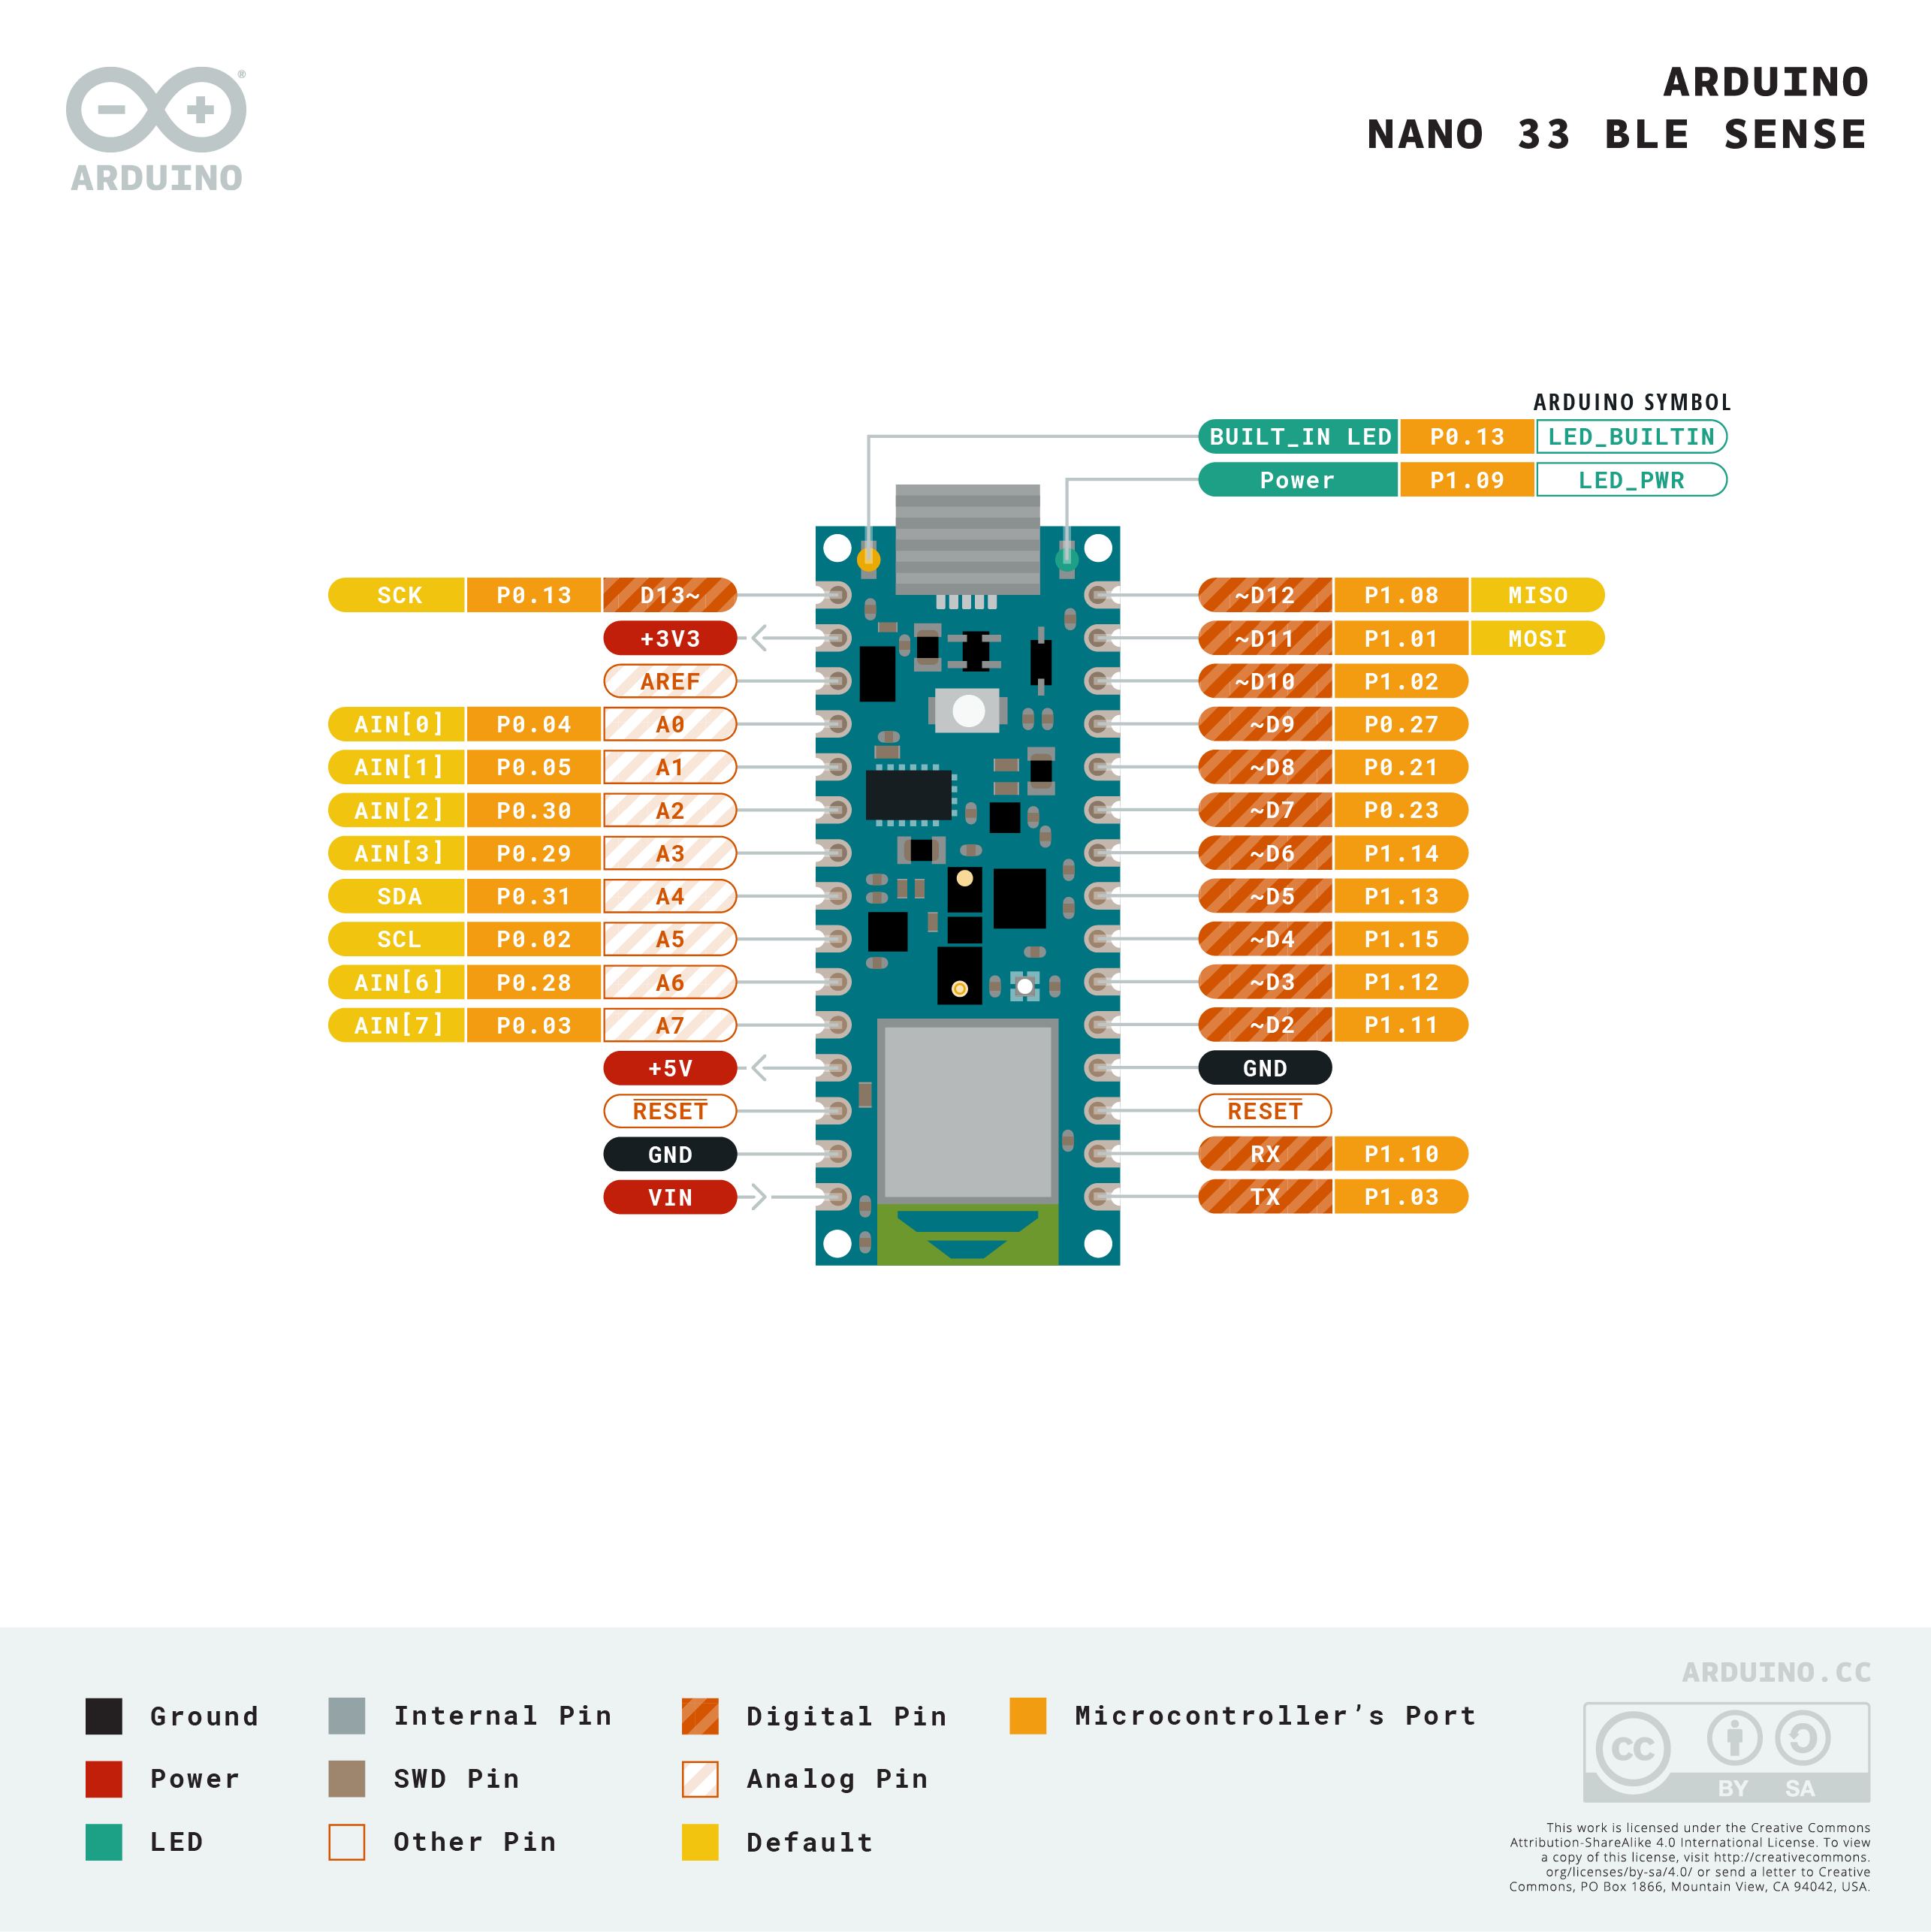
\includegraphics[width=\linewidth]{img/Pinout-NANOsense_latest.png}

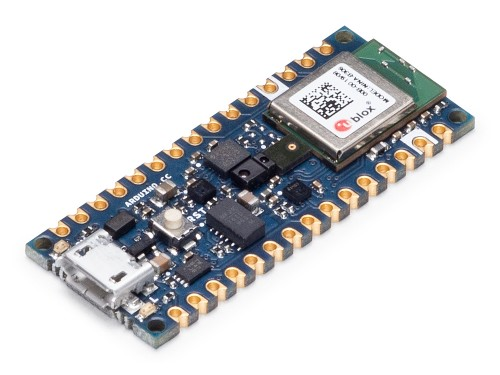
\includegraphics[width=\linewidth]{img/abx00031_iso_1.jpg}

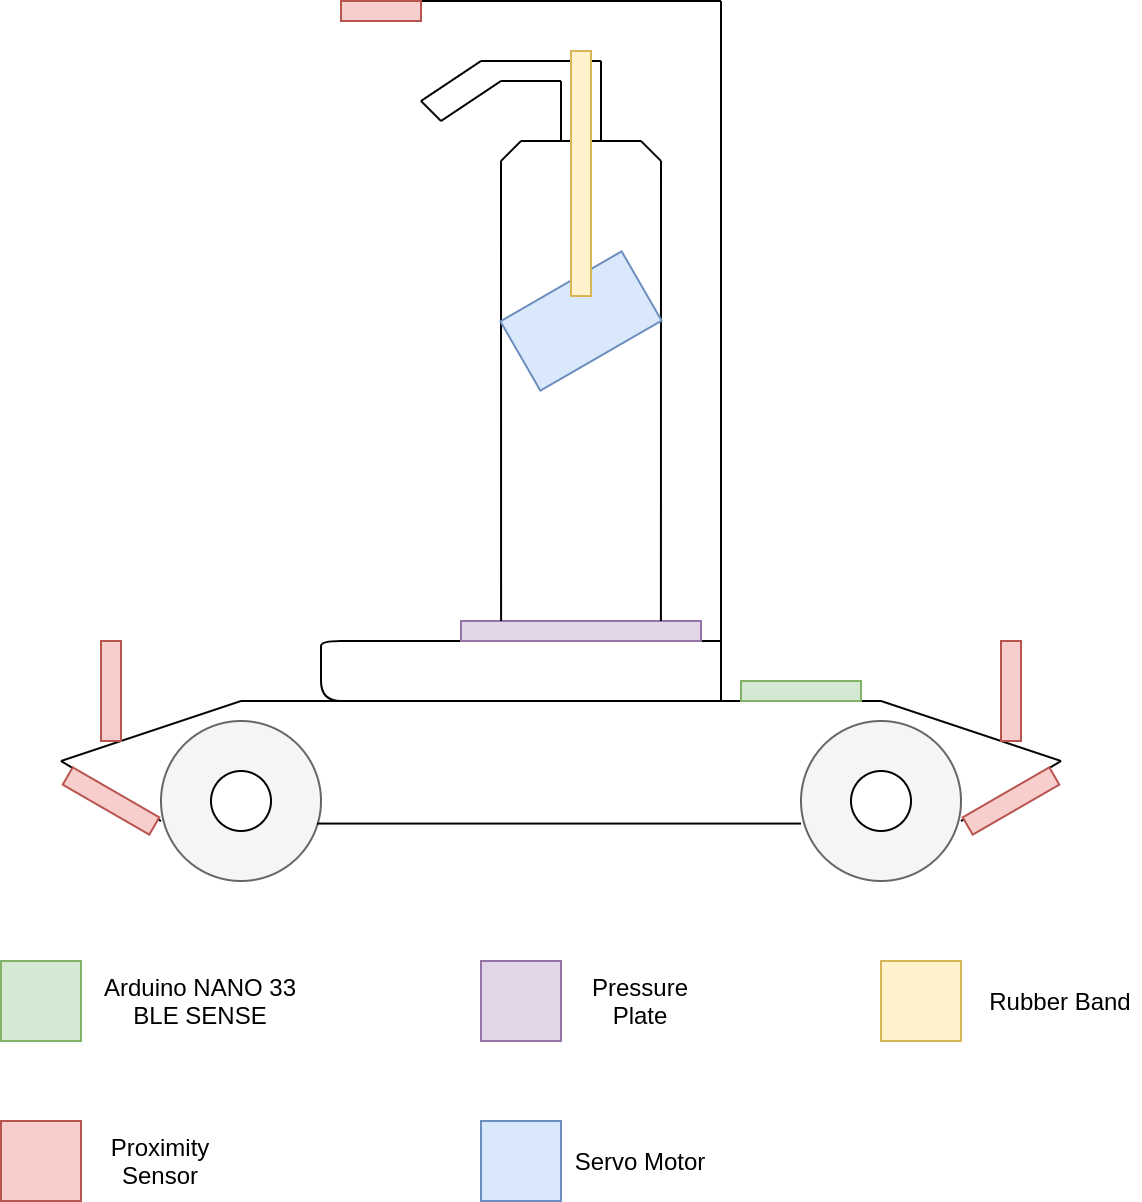
\includegraphics[width=\linewidth]{img/prototype-drawing.png}

\section{Maybe sources}

https://store.arduino.cc/arduino-nano-33-ble-sense\\
https://www.microsoft.com/en-us/hololens/buy


\end{document}

padding oracle attacks.